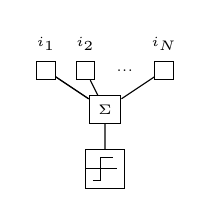
\begin{tikzpicture}[font=\tiny]

	\node (in1) at (-0.75,0) [draw,label=above:{$i_1$}]{};
	\node (in2) at (-0.25,0) [draw,label=above:{$i_2$}]{};
	\node (n) at (0.25,0) []{...};
	\node (inn) at (0.75,0) [draw,label=above:{$i_N$}]{};

	\node (sum) at (0,-0.5) [draw]{$\Sigma$};

	\node (out) at (0,-1.25) [draw,inner sep=7]{};

	\draw (out.west) --  +(0.4,0);
	\draw (out.south west) ++(0.1,0.1) -- ++(0.1,0) -- ++(0,0.3) -- ++(0.15,0);


	\draw (in1) -- (sum) -- (out);
	\draw (in1) -- (sum);
	\draw (in2) -- (sum);
	\draw (inn) -- (sum);
\end{tikzpicture}
